%% - mention standard transformation?
%%   - fission / fusion
%%   - sync removal
%%
%% - leaving out?
%%   - third-party uses?
%%     - bit-streaming / sketching
%%     - mani / VIRAM
%%   - debugging / gui's

\chapter{Optimizing StreamIt}
\label{chap:optimizing}

We demonstrate an end-to-end stream compiler that attains robust
multicore performance in the face of varying application
characteristics.  As benchmarks exhibit different amounts of task,
data, and pipeline parallelism, we exploit all types of parallelism in
a unified manner in order to achieve this generality.  Our compiler,
which maps from the StreamIt language to the 16-core Raw architecture,
attains a 11.2x mean speedup over a single-core baseline.

\section{Parallelization}

%% Our compiler relies on two new techniques.  {\it Coarse-grained data
%% parallelism} increases the granularity of data-parallel streams to
%% match the coarse-grained nature of multicores.  It is analogous to
%% fusion of DOALL loops in the scientific domain.  {\it Coarse-grained
%% software pipelining} applies traditional instruction-scheduling
%% techniques at the level of coarse-grained actors, offering a new level
%% of scheduling freedom for stream programs.  The techniques are
%% complementary and are best when applied together.

%%%%%%%%%%%%%%%%%%%%%%%%%%%%%%%%%%%%%%%%%%%%%%%%%%%%%%%%%%

%% The first technique exploits {\it coarse-grained data parallelism} by
%% duplicating data-parallel sections across cores.  While traditional
%% data parallelism incurs excessive communication and synchronization
%% costs on multicores, our technique utilizes a program analysis to
%% coarsen the granularity of data-parallel actors and duplicate them the
%% minimum number of times needed.  The second technique, {\it
%% coarse-grained software pipelining}, leverages powerful properties of
%% the stream programming model to apply traditional
%% instruction-scheduling techniques at the level of coarse-grained
%% actors.  This increases scheduling freedom and extracts valuable
%% pipeline parallelism from the application.

%%%%%%%%%%%%%%%%%%%%%%%%%%%%%%%%%%%%%%%%%%%%%%%%%%%%%%%%%%

%% In this paper, we describe two new techniques for mapping stream
%% programs to multicores.  The first technique exploits {\it
%% coarse-grained data parallelism} by duplicating data-parallel sections
%% across cores.  While traditional data parallelism incurs excessive
%% communication and synchronization costs on multicores, our technique
%% utilizes a program analysis to coarsen the granularity of
%% data-parallel actors and duplicate them the minimum number of times
%% needed.  The second technique, {\it coarse-grained software
%% pipelining}, leverages powerful properties of the stream programming
%% model to apply traditional instruction-scheduling techniques at the
%% level of coarse-grained actors.  This increases scheduling freedom and
%% extracts valuable pipeline parallelism from the application.

%% We have implemented these techniques in the StreamIt compiler,
%% targeting the 16-core Raw architecture.  Coarse-grained data
%% parallelism offers a 9.9x mean speedup over a single-core baseline,
%% while coarse-grained software pipelining offers a 7.7x speedup.
%% Combining the techniques yields the best results, achieving a 11.2x
%% speedup over a single core and 1.84x over our previous work.

Despite the abundance of parallelism in stream programs, it is
nonetheless a challenging problem to obtain an efficient mapping to a
multicore architecture.  Often the gains from parallel execution can
be overshadowed by the costs of communication and synchronization.  In
addition, not all parallelism has equal benefits, as there is
sometimes a critical path that can only be reduced by running certain
actors in parallel.  Due to these concerns, it is critical to leverage
the right combination of task, data, and pipeline parallelism while
avoiding the hazards associated with each.

\begin{figure}[t]
\centering
\psfig{figure=parallelism.eps,width=2.1in}
\caption[Types of parallelism in stream programs]{Types of parallelism
  in stream programs.  Task parallelism exists between filters in a
  common splitjoin; pipeline parallelism exists between filters in a
  producer/consumer relationship; and data parallelism exists between
  separate instances of a stateless
  filter.\protect\label{fig:parallelism}}
\end{figure}

Task parallelism refers to pairs of actors that are on different
parallel branches of the original stream graph, as written by the
programmer.  That is, the output of each actor never reaches the input
of the other (see Figure~\ref{fig:parallelism}).  In stream
programs, task parallelism reflects logical parallelism in the
underlying algorithm.  It is easy to exploit by mapping each task to
an independent processor and splitting or joining the data stream at
the endpoints.  The hazards associated with task parallelism are the
communication and synchronization associated with the splits and
joins.  Also, as the granularity of task parallelism depends on the
application (and the programmer), it is not sufficient as the only
source of parallelism.

Data parallelism refers to any actor that has no dependences between
one execution and the next.  Such ``stateless'' actors\footnote{A
  stateless actor may still have read-only state.}  offer unlimited
data parallelism, as different instances of the actor can be spread
across any number of computation units.  However, while data
parallelism is well-suited to vector machines, on coarse-grained
multicore architectures it can introduce excessive communication
overhead.  Previous data-parallel streaming architectures have focused
on designing a special memory hierarchy to support this
communication~\cite{imagine03ieee}.  However, data parallelism has the
hazard of increasing buffering and latency, and the limitation of
being unable to parallelize actors with state.

Pipeline parallelism applies to chains of producers and consumers that
are directly connected in the stream graph.  In our previous
work~\cite{streamit-asplos}, we exploited pipeline parallelism by
mapping clusters of producers and consumers to different cores and
using an on-chip network for direct communication between actors.
Compared to data parallelism, this approach offers reduced latency,
reduced buffering, and good locality.  It does not introduce any
extraneous communication, and it provides the ability to execute any
pair of stateful actors in parallel.  However, this form of pipelining
introduces extra synchronization, as producers and consumers must stay
tightly coupled in their execution.  In addition, effective load
balancing is critical, as the throughput of the stream graph is equal
to the minimum throughput across all of the processors.

In this section, we describe a robust compiler system that leverages
the right combination of task, data, and pipeline parallelism to
achieve good multicore performance across a wide range of input
programs.  Because no single type of parallelism is a perfect fit for
all situations, a unified approach is needed to obtain consistent
results.  Using StreamIt as our input and targeting the 16-core Raw
architecture, our compiler demonstrates a mean speedup of 11.2x over a
single-core baseline.  This also represents a 1.84x improvement over
our original approach~\cite{streamit-asplos}.

\subsection*{Parallelization Algorithm}

\begin{figure}[t]

\begin{minipage}{0.3\textwidth}
\centering
\psfig{figure=filterbank.eps,width=1.6in}
\end{minipage}
\hspace{0.1in}
\begin{minipage}{0.3\textwidth}
\centering
\psfig{figure=filterbank-fine.eps,width=2.2in}
\end{minipage}
\hspace{0.4in}
\begin{minipage}{0.3\textwidth}
\centering
\psfig{figure=filterbank-coarse.eps,width=1.6in}
\end{minipage}

~ \\
\begin{minipage}{0.3\textwidth}
\centering
\mbox{{\small (a) Original}}
\end{minipage}
\hspace{0.1in}
\begin{minipage}{0.3\textwidth}
\mbox{{\small (b) Fine-grained data parallelism}}
\end{minipage}
\hspace{0.4in}
\begin{minipage}{0.3\textwidth}
\hspace{-14pt}\mbox{{\small (c) Coarse-grained data parallelism}}
\end{minipage}

\centering
\caption[Mapping the FilterBank benchmark for multicore
  execution]{Mapping a simplified version of the FilterBank benchmark
  for execution on four cores.  The original stream graph is shown in
  (a), while a conventional mapping is shown in (b).  Our technique
  coarsens the graph and introduces the minimal parallelism needed, as
  shown in (c).\protect\label{fig:filterbank}}

\end{figure}

We illustrate our technique by way of an example: we discuss how to
map a simplified version of our FilterBank benchmark (see
Figure~\ref{fig:filterbank}a) to a four-core machine.  The complete
details of our algorithm are available
elsewhere~\cite{gordon06asplos}.

\paragraph*{Previous Practice: Fine-Grained Data Parallelism}  Perhaps 
the most common approach to parallelization is to identify loops that
can be run in a data-parallel (DOALL) style.  Such loops can be
annotated by the programmer using OpenMP; they are also the most
common parallelization target of production compilers.  For example,
the Intel C Compiler includes an optional flag to detect and
parallelize data-parallel loops.  In the case of FilterBank, this may
seem like a promising approach, as all the filters are stateless and
the implicit loops surrounding them can be run in a data-parallel
manner.  Figure~\ref{fig:filterbank}b illustrates such a mapping.

Unfortunately, on a coarse-grained multicore architecture, it is
hardly profitable to parallelize each individual filter due to the
communication and synchronization overheads incurred.  When we target
the 16-core Raw architecture, this approach offers only a 1.4x mean
speedup over a single core.  This represents an upper bound on the
speedups attainable using standard techniques.  In practice, for
reasons explained in Section~\ref{sec:filters}, a production C
compiler would achieve even smaller speedups due to the inherent
difficulties of proving that filters are data-parallel.

\paragraph*{First Innovation: Coarse-Grained Data Parallelism}  The
overheads of fine-grained data parallelism can be drastically reduced
by performing two novel transformations.  First, the granularity of
the stream graph is coarsened via filter {\it fusion}, a
transformation in which two neighboring filters are statically
scheduled and inlined into a single
filter~\cite{streamit-asplos,sermulins:lctes:2005}.  We fuse
neighboring stateless filters as much as possible so long as the
resulting filter remains stateless, ensuring that it is still amenable
to data parallelism.

Second, we data-parallelize the coarsened filters, but only by the
amount necessary to complement existing task parallelism in the stream
graph.  That is, for filters that are already embedded in a splitjoin,
we parallelize each filter so that the total splitjoin width covers
all of the cores, rather than data-parallelizing each branch of the
splitjoin to cover all of the cores.  By reducing the width of the
scatter and gather stages, we reduce the communication and
synchronization overhead incurred by data parallelism.

Figure~\ref{fig:filterbank}c shows an example of our
transformations on the FilterBank benchmark.  The coarsening stage
fuses all of the pipelines together with the exception of the BandStop
filter, which is not fused because it performs peeking on its input
channel.  Communication with peeking represents a case where some data
items are reused between successive firings of a filter, which would
translate to internal state if the buffer were to be inlined into a
fused filter.  Following coarsening, the parallelization stage
replicates the Adder filter across all four of the target cores.
However, the other filters are split only two ways, due to the
presence of task parallelism between alternate branches of the
splitjoin.  Applying this strategy across our benchmark suite offers a
speedup of 9.9x relative to a single core.

These transformations are out-of-reach of traditional compilers.  In
an imperative language, the analog of graph coarsening is to
selectively fuse loops so long as no new loop-carried dependences are
introduced.  The analog of task-conscious data parallelism is to
analyze the entire program for other threads that might be running
concurrently, and to introduce only as much parallelism as is needed
to complement the other threads.  We rely on the properties of the
stream programming model to make these transformations tractable.

\begin{figure}[t]
\centering
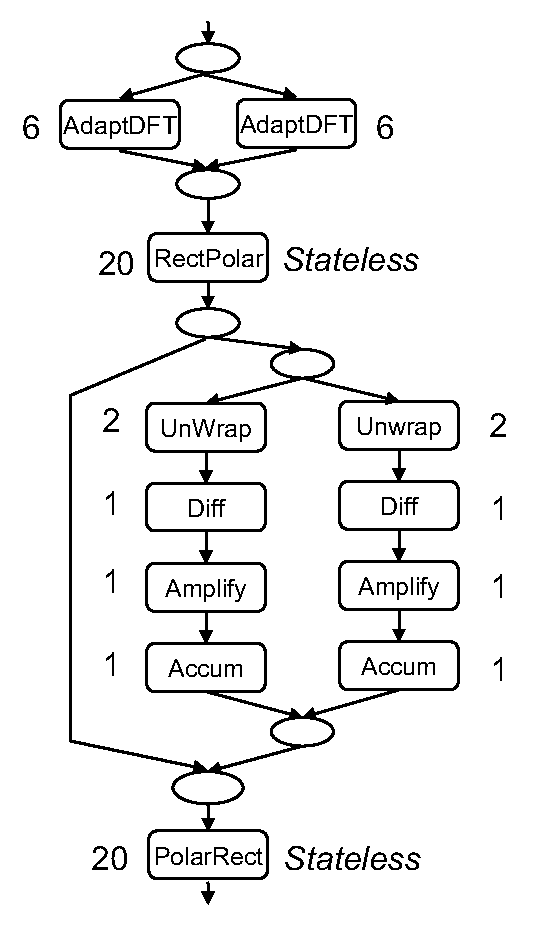
\psfig{file=vocoder.eps,width=2.25in}
\caption[Simplified subset of the Vocoder benchmark]{Simplified subset
  of the Vocoder benchmark.  Nodes are annotated with the amount of
  work that they perform per steady state.\protect\label{fig:vocoder}}
\end{figure}

\begin{figure}[t]
\centering
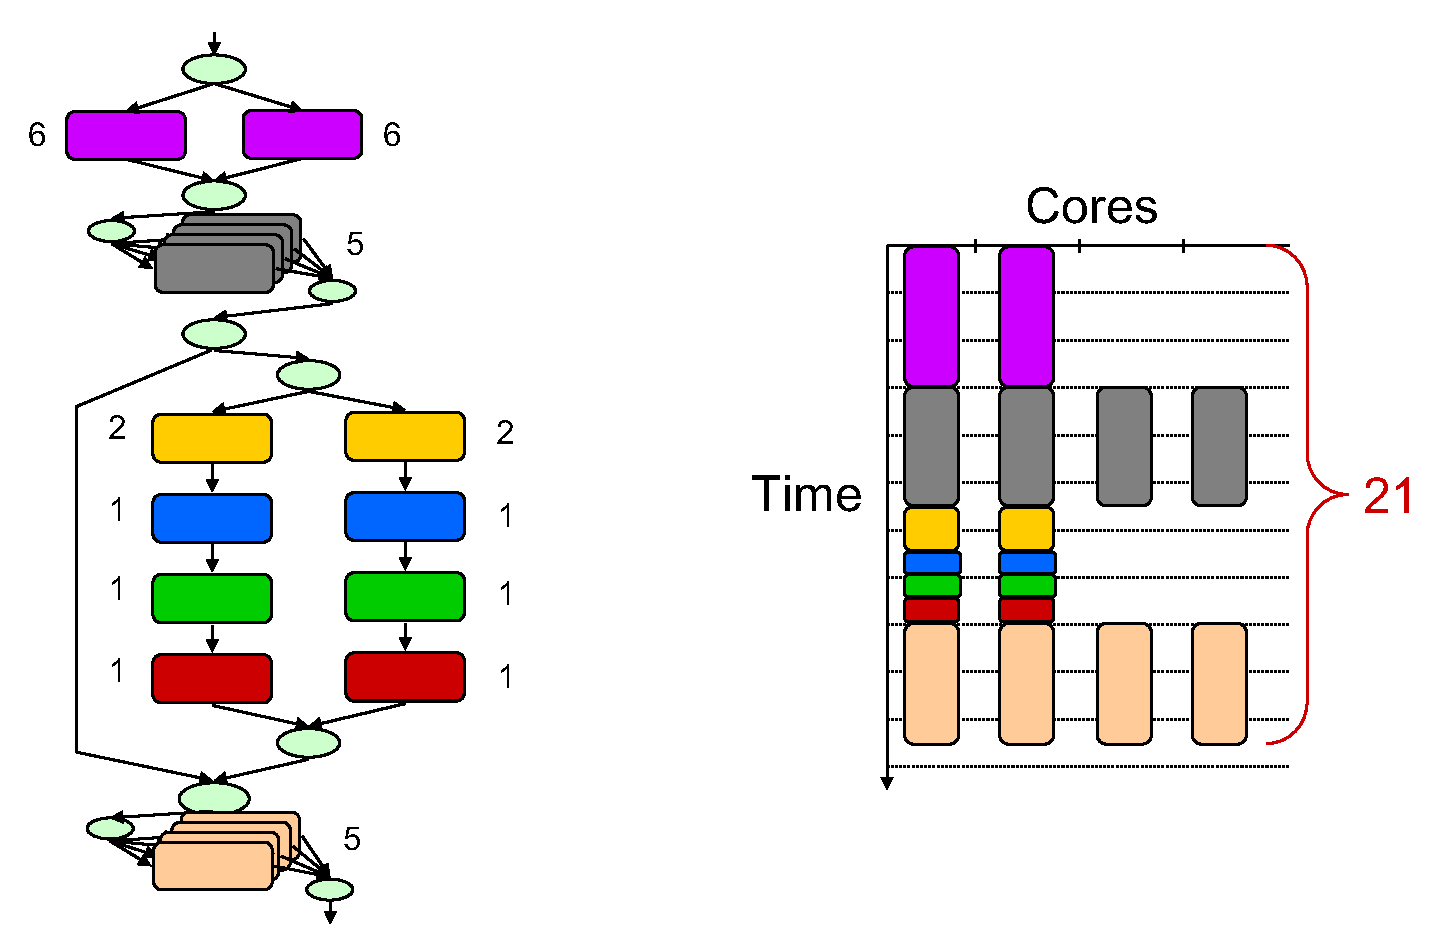
\psfig{file=vocoder-data.eps,width=4.5in}
\caption[Coarse-grained data parallelism applied to
  Vocoder]{Simplified vocoder mapped with data parallelism.  In the
  stream graph (left), stateless nodes are replicated but stateful
  nodes remain untouched.  An execution trace (right) requires 21
  units per steady state.\protect\label{fig:vocoder-data}}
\end{figure}

\begin{figure}[t]
\centering
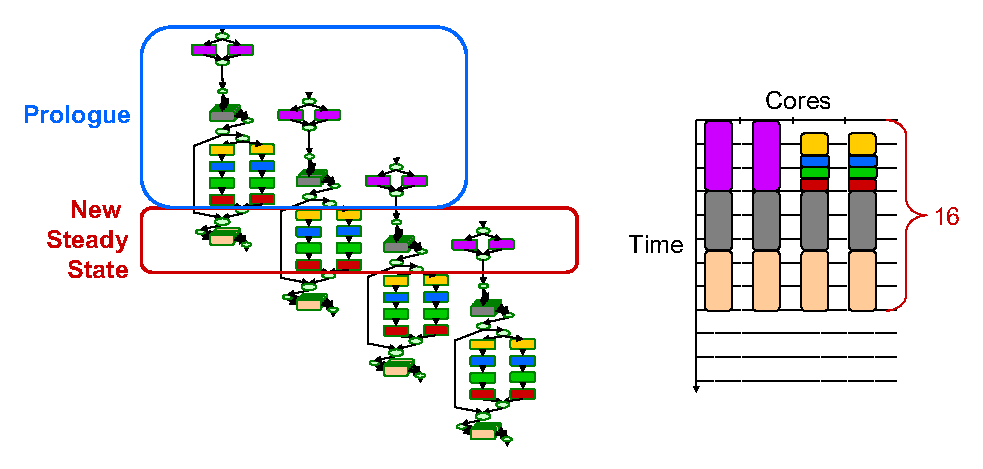
\psfig{file=vocoder-swpipe.eps,width=6in}
\caption[Coarse-grained software pipelining applied to
  Vocoder]{Simplified vocoder mapped with coarse-grained software
  pipelining.  By unrolling multiple executions of the stream graph
  (left), stateful nodes can run in parallel with other nodes during
  the steady state.  An execution trace (right) requires 16 units per
  steady state, an improvement over plain data parallelism.
  \protect\label{fig:vocoder-swpipe}}
\end{figure}

%% \begin{figure}[t]
%% \centering
%% \psfig{figure=asplos06/vocoder.eps,width=4.2in}
%% \vspace{-24pt}
%% \caption{Stream graph for a simplified subset of our Vocoder
%% benchmark.  Following a set of sliding DFTs, the signal is converted
%% to polar coordinates.  Node {\tt S2} sends the magnitude component to
%% the left and the phase component to the right.  In this simplified
%% example, no magnitude adjustment is needed.\label{fig:vocoder}}
%% \vspace{-12pt}
%% \end{figure}

\paragraph*{Second Innovation: Coarse-Grained Software Pipelining} While 
coarse-grained data parallelism is effective for parallelizing
stateless computations, it does nothing to help with computations that
retain state, either within filters or within feedbackloops.  For
example, the Vocoder benchmark (simplified subet shown in
Figure~\ref{fig:vocoder}) contains a significant fraction of stateful
filters.  While two of the filters can be data-parallelized, there
remain large gaps in the execution schedule (see
Figure~\ref{fig:vocoder-data}).
% TODO: show the real benchmark?

To run stateful computations in parallel with each other, we exploit
pipeline parallelism.  We take the concept of software pipelining,
well-understood in the context of instruction scheduling, and apply it
in the context of an entire stream graph.  As illustrated in
Figure~\ref{fig:vocoder-swpipe}, this technique involves unrolling the
execution of the graph into two stages.  In the first stage, a
prologue schedule establishes buffering in the data channels.  Then,
in the steady state, the filters are decoupled and can execute in any
order, writing intermediate results to the buffers.  Compared to
exploiting only coarse-grained data parallelism, this technique offers
large gains for our stateful benchmarks (1.7x for Vocoder, 1.9x for
Radar).  Together with coarse-grained data parallelism, it offers an
11.2x speedup over a single core across our benchmark suite.

Coarse-grained software pipelining is also beyond the reach of
traditional compilers.  Rather than pipelining individual
instructions, it represents the pipelining of entire procedures.  This
involves reordering large pieces of the program.  The stream
programming model makes such a transformation feasible by exposing the
stable flows of data between long-running actors.

\subsection*{Experimental Evaluation}

%\begin{figure}
%\centering
%\psfig{figure=asplos06/raw-diagram.eps,width=3in}
%\caption{Block diagram of the Raw architecture.
%\protect\label{fig:raw-diagram}}
%\end{figure}

We target the Raw microprocessor~\cite{raw10,raw}, a tiled array of 16
cores with a programmable mesh interconnect.  Though Raw has been
implemented in silicon, we generate results with the btl simulator,
augmented with 16 streaming DRAM controllers (providing enough
bandwidth to saturate both directions of a Raw port).  In this
configuration, one can obtain higher throughput in streaming data from
the off-chip memory than from a core's local data cache.  Thus, our
implementation elects to buffer all streaming data off-chip.  However,
when targeting an architecture with more modest off-chip memory
bandwidth, the stream buffers could reside completely in on-chip
memory.

\begin{figure}[t]
\centering
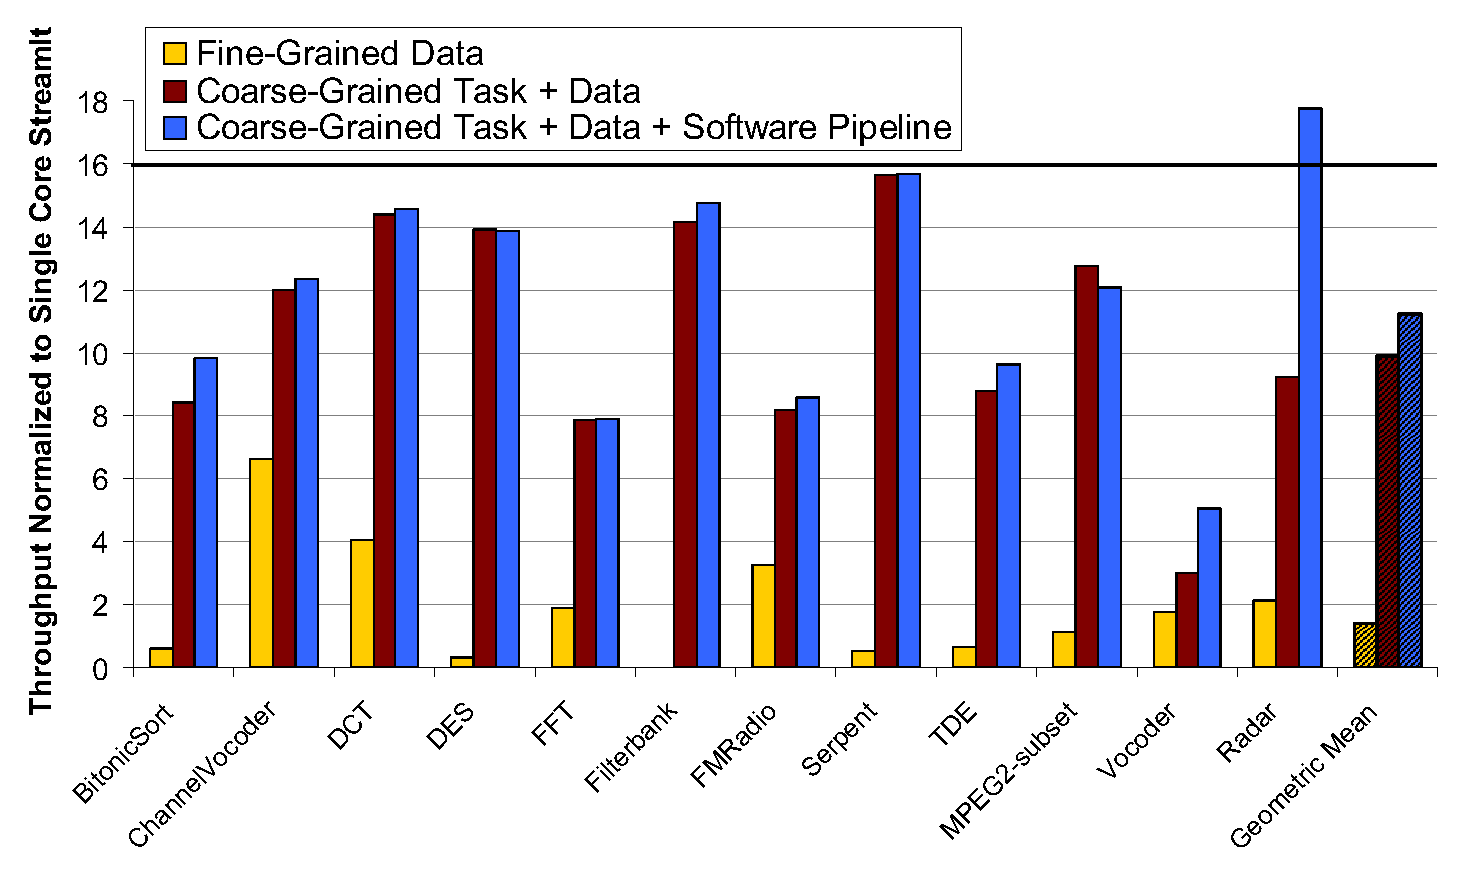
\psfig{file=par-results.eps,width=\textwidth}
\caption[Parallelization results]{Parallelization results on the
  16-core Raw processor.\protect\label{fig:par-results}}
\end{figure}

A summary of our results appears in Figure~\ref{fig:par-results}.  We
show the speedup offered by the three techniques mentioned:
fine-grained data parallelism, the previous standard; coarse-grained
data parallelism, which also leverages the existing task parallelism
in the stream graph; and coarse-grained software pipelining, which
runs as a post-pass to coarse-grained data parallelism.  Our baseline
is StreamIt executing on a single core, which (in the case of Raw) has
been shown to outperform hand-written C implementations on a single
core~\cite{raw_isca}.  While coarse-grained data parallelism performs
well (attaining a mean speedup of 9.9x), the most robust performance
comes by adding coarse-grained software pipelining (which attains a
mean speedup of 11.2x).  As expected, software pipelining mostly
benefits the stateful benchmarks, Vocoder and Radar.  There is a
super-linear speedup in Radar because reordering operations were moved
from the compute core to the network.

\subsection*{Limitations}

Our current parallelization algorithm does not support the full
generality of the StreamIt language; it omits support for teleport
messages and dynamic rates.  Messaging may constrain the latency of
certain parts of the stream graph, preventing the compiler from
exploiting data parallelism.  Also, static rates are important for
estimating the work performed by pipeline-parallel filters.  In the
software pipelining stage, static load balancing would be difficult in
the presence of dynamic rates.  Incorporating these language features
into the parallelization process is fertile grounds for future
research.

While our implementation targets Raw, the techniques developed should
be applicable to other multicore architectures.  As Raw has a
relatively high communication bandwidth, coarsening the granularity of
data parallelism may benefit commodity multicores even more.  In
porting this transformation to a new architecture, one may need to
adjust the threshold computation-to-communication ratio that justifies
data parallelism.  As for coarse-grained software pipelining, the
scheduling freedom afforded should benefit many multicore systems.
One should consider the most efficient location for intermediate
buffers (local memory, shared memory, FIFOs, etc.) as well as the best
mechanism for shuffling data (DMA, on-chip network, etc.).  The basic
algorithms for coarsening granularity, introducing data parallelism,
and software pipelining are largely architecture-independent.

%% \begin{figure}[t]
%% \centering
%% \psfig{figure=asplos06/benchchar.eps, width=6.15in}
%% \caption{Benchmark descriptions and characteristics.
%% \protect\label{fig:benchchar}}
%% \end{figure}

%% \begin{figure}[t]
%% \centering
%% \psfig{figure=asplos06/thruput.eps, width=6.1in}
%% \caption{Throughput speedup comparison and Task + Data + Software
%% Pipelining performance results.  \protect\label{fig:thruput}}
%% \end{figure}

%% \begin{figure}[t]
%% \centering
%% \psfig{figure=asplos06/maingraph.eps, width=6.5in}
%% \caption{Task, Task + Data, Task + Software Pipelining, and Task +
%% Data + Software Pipelining normalized to single core.
%% \protect\label{fig:main_comp}}
%% \end{figure}

%% \begin{figure}[t]
%% \centering
%% \psfig{figure=asplos06/fine_data.eps, width=4.5in}
%% \caption{Fine-Grained Data Parallelism normalized to single core.
%% \protect\label{fig:fine_data}}
%% \end{figure}

%% \begin{figure}[t]
%% \centering
%% \psfig{figure=asplos06/vs_space_graph.eps, width=4.5in}
%% \caption{Task + Data + Software Pipelining normalized to Hardware Pipelining.
%% \protect\label{fig:vs-space}}
%% \end{figure}

\section{Optimizing Linear Computations}

\section{Cache Optimizations}

\section{Related Work}

Liao et al. map Brook to multicore processors by leveraging the affine
partitioning model~\cite{liao06brook}.  While affine partitioning is a
powerful technique for parameterized loop-based programs, in StreamIt we
simplify the problem by fully resolving the program structure at
compile time.  This allows us to schedule a single steady state using
flexible, non-affine techniques (e.g., simulated annealing) and to
repeat the found schedule for an indefinite period at runtime.
Gummaraju and Rosenblum map stream programs to a general-purpose
hyperthreaded processor~\cite{gummaraju05micro}.  Such techniques
could be integrated with our spatial partitioning to optimize per-core
performance.  Gu et al. expose data and pipeline parallelism in a
Java-like language and use a compiler analysis to efficiently extract
coarse-grained filter boundaries~\cite{du03sc}.  Ottoni et al. also
extract decoupled threads from sequential code, using hardware-based
software pipelining to distribute the resulting threads across
cores~\cite{ottoni05decoupled}.  By embedding pipeline-parallel
filters in the programming model, we focus on the mapping step.

Previous work in scheduling computation graphs to parallel targets has
focused on partitioning and scheduling techniques that exploit task
and pipeline parallelism~\cite{SDFSched, SDFSched2,may87communicating,
DAGSched, pipeline-sdf}.  Application of loop-conscious
transformations to coarse-grained dataflow graphs has been
investigated.  Unrolling (or ``unfolding'' in this domain) is employed
for synchronous dataflow (SDF) graphs to reduce the initiation
interval but they do not evaluate mappings to actual
architectures~\cite{unfolding,unfolding2}. Software pipelining
techniques have been applied to SDF graphs onto various embedded and
DSP targets~\cite{bakshi99,chatha-02}, but has required programmer
knowledge of both the application and the architecture. To our
knowledge, none of these systems automatically exploit the combination
of task, data, and pipeline parallelism.  Furthermore, these systems
do not provide a robust end-to-end path for application
parallelization from a high-level, portable programming language.

\section{Future Work}

\section{Chapter Summary}

As multicore architectures become ubiquitous, it will be critical to
develop a high-level programming model that can automatically exploit
the coarse-grained parallelism of the underlying machine without
requiring heroic efforts on the part of the programmer.  Stream
programming represents a promising approach to this problem, as
high-level descriptions of streaming applications naturally expose
task, data, and pipeline parallelism.  

In this chapter, we develop general techniques for automatically
bridging the gap between the original granularity of the program and
the underlying granularity of the architecture.  To bolster the
benefits of data parallelism on a multicore architecture, we build
coarse-grained data-parallel units that are duplicated as few times as
needed.  And to leverage the benefits of pipeline parallelism, we
employ software pipelining techniques---traditionally applied at the
instruction level---to coarse-grained filters in the program.

A detailed evaluation in the context of the StreamIt language and the
16-core Raw microprocessor offers very favorable results that are also
quite consistent across diverse applications.  Coarse-grained data
parallelism offers a 4.4x speedup over a task-parallel baseline and a
9.9x speedup over a sequential code.  Without our granularity
coarsening pass, these reduce to 0.7x and 1.4x, respectively.
Coarse-grained software pipelining improves the generality of the
compiler, as it is able to parallelize stateful filters with
dependences from one iteration to the next.  Our two techniques are
complementary and offer a combined speedup of 11.2x over the baseline
(and 1.84x over our previous work).

As our techniques rely on specific features of the StreamIt
programming model, the results suggest that these features are a good
match for multicore architectures.  Of particular importance are the
following two language features:
\begin{enumerate}
\item Exposing producer-consumer relationships between filters.  This
enables us to coarsen the computation to communication ratio via
filter fusion, and also enables pipeline parallelism.

\item Exposing the outer loop around the entire stream graph.  This is
central to the formulation of software pipelining; it also enables
data parallelism, as the products of filter fission may span multiple
steady-state iterations.
\end{enumerate}

%% - lessons learned
%%   - fine-grained communication on Raw not worth it
%%   - greedy is good?  dynamic programming solution
%%   - what was useful in language for compiler's sake?
%%    - peeking was useful for compiler
%%    - data reordering was useful for compiler
%%    - structure was less useful for compiler
%%      - mostly just dynamic programming solution
%%      - phased scheduling was easier to formulate
%%      - COULD have been useful for parameterized IR

